%%
% TUM Corporate Design LaTeX Templates
% Based on the templates from https://www.tum.de/cd
%
% Feel free to join development on
% https://gitlab.lrz.de/tum-templates/templates
% and/or to create an issue in case of trouble.
%
% tum-article class for scientific articles, reports, exercise sheets, ...
%
%%

\documentclass[twocolumn]{tum-article}
%\documentclass[twocolumn, german]{tum-article}
%\documentclass[times, twocolumn]{tum-article}
%\documentclass[times]{tum-article}
%\documentclass{tum-article}

\usepackage{lipsum}

\title{Modifying the Writing Style in Goal-Oriented Dialog Generation}
\author{Fabian Bell\authormark{1,\Letter}\orcid{0000-0001-9595-4226},
  Monika Wintergerst\authormark{1}\orcid{0000-0002-9244-5431}}

% if too long for running head
\titlerunning{TUM Article}
\authorrunning{Author 1 et al.}

\email{fabian.bell@tum.de}

\affil[1]{Department of Informatics, Technical University of Munich (TUM),
  Boltzmannstr. 3, 85748 Garching, Germany}

\begin{document}

\maketitle

\begin{abstract}
In this work we evaluate the usage of Soloist in combination of TextSETTR or DGST in order to modify the style of the dialogue agents response. We show that the Soloist yields reasonable performance in a significantly smaller setup. Further, we show that the TextSETTR performance cannot be reproduced on the Fine-Food dataset, not merged with Soloist, not independent in a smaller setup, nor as the original approach. Additionally, we show that the LSTM-DGST performance cannot be reproduced either given the Donald Trump twitter dataset. We release our code as well as the pre trained reduced Soloist model. 
\end{abstract}

\section{Introduction}\label{sec:intro}

Dialogue systems (e.g. Chat-bots) have made great progress during the last years, mainly due to the invention of novel neural models and machine learning techniques. Because of the progress, current research aims to improve the dialogue systems on an individual and human-like level. Recent articles \cite{DBLP:journals/corr/abs-1901-08149, liu2020impress} tried to tackle this problem by feeding a persona into the network. The network is then trained to extract characteristic information from the given persona in order to generate a human-like output sequence. The persona is defined by a set of profile sentences like "\textit{I like books}". The problem of these approaches consist of two tasks:
\begin{itemize}
\item \textbf{Persona understanding:}\\
The network needs to understand what the characteristics of the given persona are. This also yields the question on what defines a certain persona and on how to formulate the profile sentences, since the persona definition has to be done manually. 
\item \textbf{Style derivation:}\\
The network needs to derive a certain speaking/writing style from the given persona. Profile sentences like "\textit{I bought my first home}" \cite{liu2020impress} do not necessarily contribute to a distinct writing style.
\end{itemize}
An alternative approach is to extract the style in an abstract representation from given context sentences in order to infuse the style in the response generation process of a dialogue agent. With the ability to extract style from an arbitrary context we are able to create the context automatically or let it be generated by the user, thereby we do not need hand crafted pre-defined styles but are able to react to a style more dynamically. A recent attempt called TextSETTR \cite{riley2020textsettr} tries to perform abstract style extraction from an arbitrary context. An additional advantage of \cite{riley2020textsettr} is that they use a collection of self supervised train tasks in order to train TextSETTR. This enables the possibility to easily generate a large amount of suitable data and moreover, consider a significantly larger variance of different writing styles from different sources. 
An alternative approach is the DGST model \cite{li2020dgst}. This approach is restricted to only a transformation between two given styles. The resulting model is again trained on a self supervised training task.\\
Traditionally, a goal oriented dialogue agent consists of three components a (1) \textit{natural language understanding} unit (NLU), a (2) dialogue management unit and a (3) \textit{natural language generation} unit (NLG). The NLU unit extracts information from the dialogue and presents them in a predefined format by slot filling. The dialogue management unit contains a state tracker that keeps track of the dialogue history as well as the user goal. Together with the user goal and the extracted information we can then query additional data from a database. Based on the previous information the dialogue management then decides the next action with a learned policy. The NLG unit then generates the systems response conditioned on the previous information and the next action.\\
Training these units can be quite labour intensive. All units have to be trained individually. Specifically, the policy function of the dialogue management unit requires a lot of additional work. Usually, the policy function is trained via reinforcement learning \cite{DBLP:journals/ml/Williams92}. Since a dialogue is a non-deterministic environment the reinforcement signal has to be generated by a human, which can be quite time intensive. Recent work has shown that this work can be reduced by introducing a trainable model that tries to generate the reinforcement signal automatically \cite{DBLP:journals/corr/abs-1907-00448}. However, this approach still requires at least some human interaction in order to train the model that should generate the signal.\\
\begin{figure*}[!h]
\centering
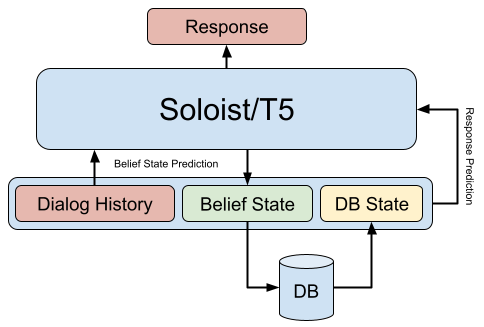
\includegraphics[width=0.8\textwidth]{figures/Soloist.png}
\caption{Soloist approach \cite{peng2020soloist}. Instead of using the GPT-2 Model \cite{radford2019language}, we use the T5 Model \cite{raffel2019exploring}.}
\label{fig:soloist}
\end{figure*}
Due to recent progress in sequence-to-sequence (seq2seq) models \cite{radford2019language, raffel2019exploring} current work tries to fuse the NLU, dialogue management and NLG units into one seq2seq model like in \cite{peng2020soloist}. \\
In this work we will evaluate state-of-the-art models like Soloist, TextSETTR and DGST in a smaller, more commonly usable setup. Further, we will evaluate two combined models from the Soloist and TextSETTR models. We will evaluate 
\begin{enumerate}
\item Merged Soloist and TextSETTR
\item Soloist and TextSETTR with shared weights
\end{enumerate}
\section{Theory}
In this section we introduce the different approaches. We will briefly describe the methods the approaches use as well as the different training tasks. 
\subsection{Soloist}\label{sec:soloist}
The \textit{Soloist} \cite{peng2020soloist} approach fuses the different units into two seq2seq steps that are executed sequentially as shown in \autoref{fig:soloist}. In the first step, the previous dialogue history is used to predict the next belief state. The belief state is then parsed and transformed into a suitable format for the given knowledge base. The response of the knowledge base is then concatenated with the dialogue history and the belief state. The concatenation is fed into the model again in order to predict the next system response.\\
The dataset that is used in \cite{peng2020soloist} is the MultiWOZ dataset \cite{budzianowski2020multiwoz}. The MultiWOZ dataset is a multi domain dialogue dataset consisting of 6 different domains. Based on that dataset Authors introduced three different training tasks:
\begin{enumerate}
\item \textbf{Belief Prediction}\\
The belief state is predicted as a seq2seq task. Thereby, the loss is calculated by the cross entropy loss of the target belief state sequence and the predicted belief state sequence.  
\item \textbf{Ground Response Generation}\\
The response generation is again a seq2seq task and uses the same criterion than the previous task.
\item \textbf{Contrastive Objective}\\
Beside optimising the similarity of the predicted and the ground truth sequences it is an essential part of the agent to place the correct information in the respective slots in the belief state or response. The authors therefore suggest a task that tries to enhance the awareness of the model towards incorrect target sequences. For that they sample normal target sequences from the MultiWOZ dataset, as well as corrupted target sequences where the key information (eg. theatre location, movie name) is replaced by a random key information from the dataset. Based on the samples they apply a binary classification given the output of the models encoder to predict if the sequence is corrupted or not. The loss is calculated by the binary cross entropy loss. 
\end{enumerate}
\subsection{Soloist Modifications}
\label{sec:soloist_mod}
\begin{figure*}[!h]
\centering
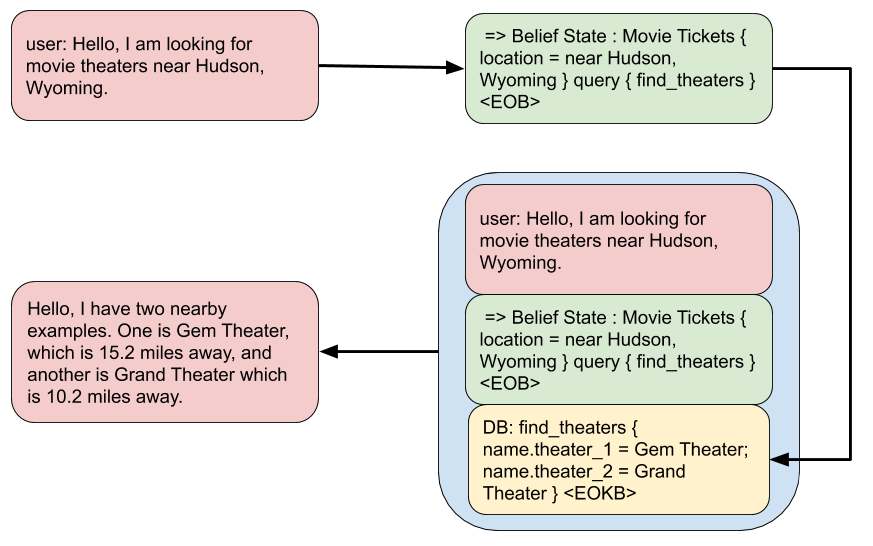
\includegraphics[width=0.8\textwidth]{figures/Soloist_Data.png}
\caption{An example in the format of \cite{peng2020soloist} with additional query word.}
\label{fig:soloistdata}
\end{figure*}
Due to resource limitations we decided to scale down the model described in \cite{peng2020soloist}. The authors implementation is based on the GPT-2 Model\cite{radford2019language} implemented by the Huggingface Transformers\cite{wolf2019huggingface}. In order to reduce the required resources we decided to take the T5-small\cite{raffel2019exploring} model. The GPT-2 Model has 117M parameters whereas T5-small has only 60M parameters\footnote{\url{https://huggingface.co/transformers/pretrained_models.html}} but still performs reasonably well.
Additionally, we modified the \textit{Belief State Prediction} task by adding an additional query word to the target sequence. The query word is used to properly transform the belief state to a format that can be used to query data from the knowledge base. An example of modified format is shown in \autoref{fig:soloistdata}. 
\subsection{TextSETTR} \label{sec:textsettr}
The \textit{TextSETTR} \cite{riley2020textsettr} approach tries to model the style transfer task a noisy reconstruction task. The model gets as a noisy, corrupted sentence, as well as a normal sentence from the same style as the fist sentence. The model then has to reconstruct the first sentence. The theory behind this approach is that the model extracts and uses the style of the second sentence in order to reconstruct the first sentence.\\
The model is based on the T5 large Model with an additional encoder used for extracting the style based on the reference sentence. The resulting model has 1 billion parameters. Following \cite{devlin-etal-2019-bert, raffel2019exploring} a style vector $v$ is extracted based on the reference sentence embeddings by using the embedding of the "[CLS]" token. The style vector $v$ is the added to the embedding of the input sentence token wise. The T5 decoder is trained on a large and diverse dataset \cite{raffel2019exploring}, therefore based on \cite{riley2020textsettr} the decoder should entail a lot of knowledge of different writing styles and should be able to understand and interpret the different style representations.\\
The dataset that is used in \cite{riley2020textsettr} is the amazon review dataset \cite{li2018delete}. For corrupting the data they use two types of corruption methods:
\begin{enumerate}
\item \textbf{Noise}:\\
This methods corrupts input by dropping random tokens or by replacing tokens by a random token by a token from the dataset. For replacing the $k$-th token in sentence $s_1$, a different sentence $s_2$ is sampled from the dataset. The token is then replaced by the $k$-th token in sentences $s_2$. A sentences is first corrupted by dropping tokens and then by replacing tokens. For each sentence a noise probability $p$ is sampled from a uniform distribution in the range $20-40\%$. A token is then dropped/replaced by the probability $p$ independently but sequential.
\item \textbf{Back translation}:\\
For applying back translation on sentence $s_1$ a sentence $s_2$ from the dataset is sampled where $s_1$ and $s_2$ do not have the same style. The model is then applied on $s_1$ with $s_2$ as the reference sentence. The resulting sentence is then taken as corrupted sequence of $s_1$. 
\end{enumerate}
Based on these two corruption method \cite{riley2020textsettr} derive the respective reconstruction tasks as described above. The final loss is the sum of the task specific losses. 
An additional idea of \cite{riley2020textsettr} approach is to control how eager the model replaces or adapts token in the translation process. Therefore they prepend the input sequence embeddings with the vector $(a_1, a_2, d_1, d_1, 0, \dots, 0)$ of length $d\_model$, where $d\_model$ is the embedding dimension. $(a_1, a_2)$ and $(d_1, d_2)$ represent the range of \textit{added} and \textit{deleted} tokens, respectively. The true value of added and deleted tokens lies within these ranges and the range as well as the center of the ranges is sampled randomly.\\
\begin{figure*}[!h]
\centering
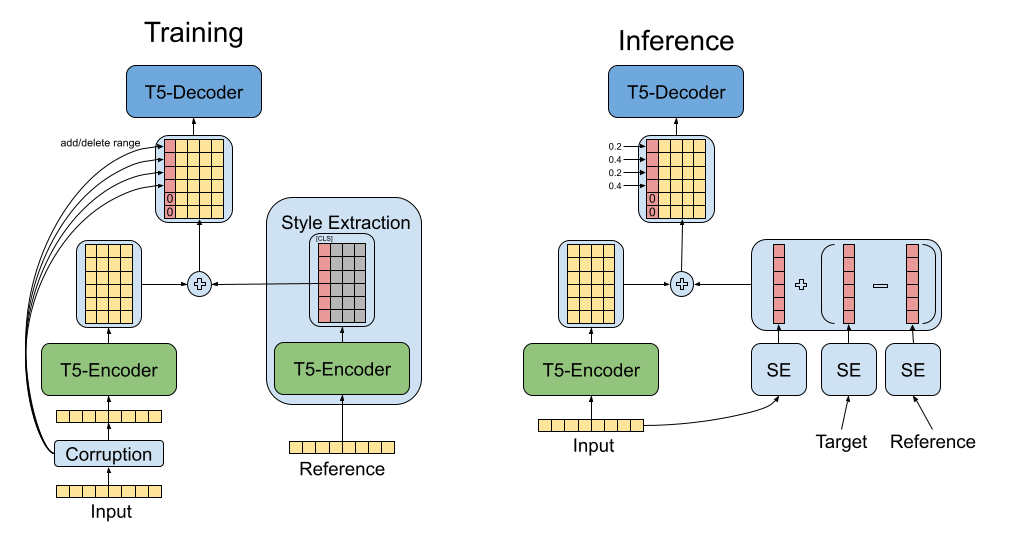
\includegraphics[width=\textwidth]{figures/TextSETTR.png}
\caption{The text TextSETTR Model \cite{riley2020textsettr} in training and inference mode}
\label{fig:textsettr}
\end{figure*}
In case of inference following \cite{riley2020textsettr} the input sentence is not corrupted but perceived to be corrupted by a different style like in the back translation corruption method. The computation of the style vector differers from the computation of the style vector in the training case. Let $f$ be the style encoding, $s_1$ the input sentence, $s_2$ a sentences from the target style and $s_3$ sentence form the same style as $s_1$, then the style vector $v$ is computed as $v = f(s_1) + (f(s_2) - f(s_3))$. Since the input is not actually corrupted the \textit{add} and \textit{delete} rates are both set to $20\%-40\%$. A visualisation of the model in training and inference mode is shown in \autoref{fig:textsettr}.
\subsection{Small TextSETTR}\label{sec:textsettr_small}
Since the Model described by \cite{riley2020textsettr} results in a model with 1 billion parameters it very hard to train and requires an enormous amount of hardware resources for training as well for production. Similar to the modified Soloist as described in \autoref{sec:soloist_mod} we can reduce the model from T5-large to T5-small for the decoder and both encoder in the TextSETTR approach. This results in a model with \textbf{TODO} parameter, which is significantly easier to work with. 
\subsection{Soloist and TextSETTR as merged models}
In an alternative computationally less expensive variation we try to merge the Soloist and TextSETTR by letting the decoder and the main encoder be shared between both models. The main encoder in the TextSETTR model is the encoder that processes the corrupted sentence but not the style extractor (see \autoref{fig:textsettr}). Analogue to \autoref{sec:soloist_mod} and \autoref{sec:textsettr_small} instead of using the GPT-2 model or T5-large, respectively, we take the T5-small model. The resulting model has \textbf{TODO} parameters. We train the model by concatenating the list of tasks from both approaches. The loss of both approaches is weighted equally in our final loss function. Let $l_1$, $l_2$ and $l_3$ be the losses from the Soloist tasks described in \autoref{sec:soloist} and let $l_4$ and $l_5$ be the tasksed derived by the corruption methods described in \autoref{sec:textsettr}, then our final loss is computed as:
$$
loss = \frac{1}{3}(l_1 + l_2 + l_3) + \frac{1}{2} (l_4 + l_5)
$$
Since every task is a seq2seq task we can compute all task together in one batch. However, the TextSETTR approach prepends the embedding dimension with vector $v$ that indicates the corruption range of the sentence as described in \autoref{sec:textsettr}. Therefore, we have to prepend the embeddings of the Soloist tasks sentences as well to make the batch a valid tensor again. To avoid that the prepended vector is accounted in the soloist tasks we want to set the attention masks accordingly as described in \cite{vaswani2017attention}. The classifier used for the soloist task "\textit{Contrastive Objective}" as described in \autoref{sec:soloist} is not used by the TextSETTR part.
\subsection{DGST}
As mentioned in \autoref{sec:intro} an alternative approach is the DGST model \cite{li2020dgst}. This approach is limited to the style transfer between two given styles and cannot be changed after training. The DGST approach is again based on a noisy reconstruction task. Let $S_1$ and $S_2$ be two different styles, then DGST uses two different seq2seq models $g_1$ and $g_2$, in order to transfer a text between the different styles as $g_1: S_1 \rightarrow S_2$ and $g_2: S_2 \rightarrow S_1$. Both generators are trained jointly. As a corruption method the authors define the set $U(y, \gamma)$, which is the set with all modifications of $y$ with noise intensity $\gamma$. The noise intensity is the mean of a folded normal distribution $\mathcal{F}$. The authors construct $U(y, \gamma)$ by sampling $m$ from $\mathcal{F}$ and add all sentences $y'$ to $U(y, \gamma)$ with $m$ modifications. A modification here means either a replacement, a deletion or an insert of a token. Let $n$ be the described noise function and let $x, y$ be text from the styles $S_1$ and $S_2$, respectively, then $g_1$ is trained by optimising 
$$
\mathcal{L}_{g_1} = \mathcal{L}(x, g_1(n(x), \Theta_1)) + \mathcal{L}(x, g_1(n(g_2(x, \Theta_2)), \Theta_1))\textnormal{.}
$$
The loss function $\mathcal{L}$ computes the cross entropy loss of the generated sequences. When training $g_1$ we do not update the parameters $\Theta_2$. The $g_2$ is trained analogously.The final loss is the sum of $\mathcal{L}_{g_1}$ and $\mathcal{L}_{g_2}$.
\section{Experimental Setup}\label{sec:experiment_setup}
In this section we describe the different training setups. This includes the datasets and hyperparameters that are used, as well as the used hardware.
\subsection{Soloist Setup}\label{sec:soloist_setup}
\begin{figure}[!h]
\centering
\begin{tabular}{c|c|c}
\hline
\textbf{Statistic} & \textbf{Taskmaster} & \textbf{MultiWOZ}\\
\hline
\# unique words & 21,894 & 19,175 \\
\hline
\# unique names entities & 8,218 & 1,338 \\
\hline
Perplexity & 17.08 & 15.62 \\
\hline
BLEU & 6.53 & 11.02\\
\hline
\end{tabular}
\caption{Dataset comparison from \cite{byrne2019taskmaster}.}
\label{fig:taskmaster}
\end{figure}
Similar to the MultiWOZ dataset \cite{byrne2019taskmaster} introduced the Taskmaster dataset. As stated by the authors the Taskmaster dataset has a richer and more diverse language than the MultiWOZ dataset as shown in \autoref{fig:taskmaster}. Due to resource limitations and due to the smaller model that is used in this work we decided to only select one domain for training and validation. Since the Taskmaster is more rich as the MultiWOZ dataset and the dataset is more easy to process we decided to train on a subdomain of the Taskmaster dataset. The selected domain from the Taskmaster dataset is the \textit{Movie Ticket} domain, where the system has to guide the user through the ordering process. 

The model was trained with free available resources provided by Google Colab\footnote{\url{https://colab.research.google.com/}}. Specifically, we trained on a Tesla T4\footnote{https://www.nvidia.com/de-de/data-center/tesla-t4/}, which, at the time of writing, is the most commonly assigned GPU at google colab. We used the hyper parameters provided by \cite{peng2020soloist} and trained until convergence. Since the authors do not report a learning rate but refer to \cite{kingma2014adam}, we assume they choose the default setting which is $1e-3$. 
\subsection{Small TextSETTR setup}\label{sec:textsetter_small_setup}
When working with only limited resources, an additional problem that occurs when following \cite{riley2020textsettr} is working with the dataset proposed by the authors. The dataset that is used in the TextSETTR approach is the "\textit{Amazon Review Dataset}" \cite{ni2019justifying}. This dataset consists of 233.1 million reviews, which requires 34 GB of storage space. Even though \cite{riley2020textsettr} discards single line reviews the remaining data is still difficult to work with. Analogue to \autoref{sec:soloist_setup} we reduce the data to only specific domain. Therefore, we train the model on the "\textit{Fine Food Dataset}" \cite{mcauley2013amateurs} with $500.000$ amazon reviews from the food domain. We use the hyper parameters provided by \cite{riley2020textsettr}. Since, we cannot fit the required batch size of $65,536$ tokens on the given GPU we apply the accumulated gradient method accordingly. 
\subsection{Merged Soloist-TextSETTR setup}\label{sec:soloist_textsettr_setup}
Analogue to \autoref{sec:textsetter_small_setup} and \autoref{sec:soloist_setup} we use the reduced datasets "\textit{Taskmaster}" and "\textit{Fine Food}". We choose a batch size of $65,536$ according to the TextSETTR approach (with accumulated gradients), a learning rate of $1e-3$ and we train for $100$k steps, which is the maximum number of steps from both approaches. We train on a Tesla K80\footnote{\url{https://www.nvidia.com/de-de/data-center/tesla-k80/}}.
\subsection{TextSETTR Setup}
Training the original TextSETTR cannot be reproduced with publicly available resources like those provided by google colab, due to the enormous amount of 1 billion parameters. The model does not fit in the GPU RAM of the GPUs provided by google colab (at the time of writing). Therefore, we distribute and compute the model layers on multiple devices in order to fit the partial model as well as the data that is produced during computation into the GPUs RAM. We train on 4 Tesla K80 and use the parameters provided by \cite{riley2020textsettr} with accumulated gradients. Again, we use the reduced "Fine-Food" dataset. 
\subsection{DGST Setup}
The DGST setup allows any seq2seq model as the respective generators. Since the reported results in \cite{li2020dgst} are based on a 4-layer BiLSTM we adapted the model choice in our experiments. Despite what is written in \cite{li2020dgst} the code\footnote{\url{https://github.com/lissomx/DGST/blob/30438e24a3c6b2abe8ceeda214863fcf79cf379f/Exp\_DGST.py\#L104}} published by the authors show a different implementation of the corruption method. They restrict the token modifications for $U(y, \gamma)$ to replacement operations only. We adapt this in our experiment. The results published in \cite{li2020dgst} are based on the Yelp\cite{li2018delete}. The Yelp dataset task is based on sentiment swapping. As described in \autoref{sec:intro}, we are more interested in modifying the writing style rather than changing the content of a utterance. Therefore, we use the messages from the twitter account of Donald Trump as our training data. We use the data published by thetrumparchive\footnote{\url{https://www.thetrumparchive.com/}}. We use the hyper parameters provided by the authors and again train on a Tesla T4 gpu. Analogue to \cite{li2020dgst} we train until convergence and reduce $\gamma$ from $0.3$ to $0.03$. After that we repeat the training until convergence.     
\section{Results}
In this section we present the results of the experiments that are introduced in the previous section.  
\subsection{Soloist Result}
\begin{figure*}[!h]
\centering
\begin{tabular}{c|c|c|c|c|c|c}
\hline
\textbf{Model} & \textbf{\# Parameters} & \textbf{Dataset} & \textbf{Inform} & \textbf{Success} & \textbf{BLEU} & \textbf{Combined}\\
\hline
Soloist(large) & 117M & MultiWOZ(full) & 85.50 & 72.90 & 16.54 & 102.49 \\
\hline
Soloist(small) & 60M & Taskmaster(Movie Tickets) & 84.24 & 67.30 & 60.79 & 136.56\\
\hline
\end{tabular}
\caption{Results of the Soloist experiment. The models are not evaluated on the same dataset nor on the same domain but on the same overall tasks. Thus the models cannot be compared directly. }
\label{fig:soloist_res}
\end{figure*}
Due to our resource limitations we could not follow \cite{peng2020soloist} directly but we had to reduce the approach to a smaller model on a smaller domain as described in \autoref{sec:soloist_mod}. Thereby the results stated in \autoref{fig:soloist_res} cannot be compared directly. 
We follow the automatic evaluation as in \cite{peng2020soloist, budzianowski2020multiwoz}. The \textit{inform rate} measures if the model predicts a correct entity. An entity is a combination of a slot (e.g. location) and a slot value (e.g. Munich). The \textit{success rate} measures if the system provides all the requested information. The combined score is computed as $Combined = (Inform + Success) \times 0.5 + BLEU$.
Due to the smaller domain the model performs better on the \textit{BLEU} score, however, performs worse on the \textit{Inform} and \textit{Success} score. Because of the higher \textit{BLEU} score the \textit{Combined} score is higher as well. 
The high \textit{BLEU} score can be explained by the significantly smaller vocabulary domain in which the small model has to perform. As described in \autoref{sec:soloist_mod} we tried to counteract this problem by choosing a more rich dataset with a lower BLEU score.  
\section{TextSETTR Results}
\textbf{TODO}
\section{DGST}
\textbf{TODO}
\section{Conclusions}
We have shown that the \textit{Soloist} model performs well with a significantly smaller setting on a single domain dataset. In many industry use cases the dialogue task is more limited to a very specific language domain as well as to a very specific task domain. For these use cases we have shown that the development cost as well as the production costs can be reduced by using a smaller version of the Soloist model and still achieve reasonable performance. Additionally, we have shown that the TextSETTR model with the configurations described in \autoref{sec:experiment_setup} cannot be used with the "Fine-Food" dataset in order to achieve a proper style modification. The same holds for the DGST approach on the Donald Trump dataset.
\section{Future Work}
In future work one might focus on a style transfer models that require significantly smaller setup. This would open up the usage of style transfer for research with limited resources as well for many industry applications where a resources consumption of models like TextSETTR might not be feasible.
\section*{Acknowledgements}
We want to thank Pyoneer\footnote{\url{https://www.pyoneer.io/}} for providing us with additional resources to try out the TextSETTR approach. 
\bibliographystyle{apalike}
\bibliography{literature}
\end{document}
